\documentclass[a4paper,12pt]{article}

\usepackage{cmap}					% поиск в PDF
\usepackage[T2A]{fontenc}			% кодировка
\usepackage[utf8]{inputenc}			% кодировка исходного текста
\usepackage[english,russian]{babel}	% локализация и переносы
\usepackage{enumitem}  				% смена типа символя у enumerate
\usepackage{amsmath,amsfonts,amssymb,amsthm,epsfig,epstopdf,titling,url,array}
\usepackage{icomma} 				% "Умная" запятая: $0,2$ --- число, $0, 2$ --- перечисление
\usepackage{hyperref}				% кликабельные ссылки
\usepackage{soulutf8} 				% Модификаторы начертания


\usepackage[backend=biber,
			bibencoding=utf8,
			maxcitenames=2,
			style=authoryear]	
		{biblatex}					% библиография

\addbibresource{sources.bib}

\newtheorem{theorem}{Теорема}[section]
\newtheorem{corollary}[theorem]{Следствие}


\theoremstyle{definition}
\newtheorem{property}{Свойство}[subsection]
\renewcommand\theproperty{\arabic{property}}

\usepackage[shortcuts]{extdash}

\graphicspath { {img} }

\sloppy

\title{Исследование поточного алгоритма шифрования типа «Раскольников» \linebreak Вариант №4.}
\author{Роман Астраханцев, СКБ-171}

\begin{document}
	\maketitle
	
	\section*{Описание алгоритма}

	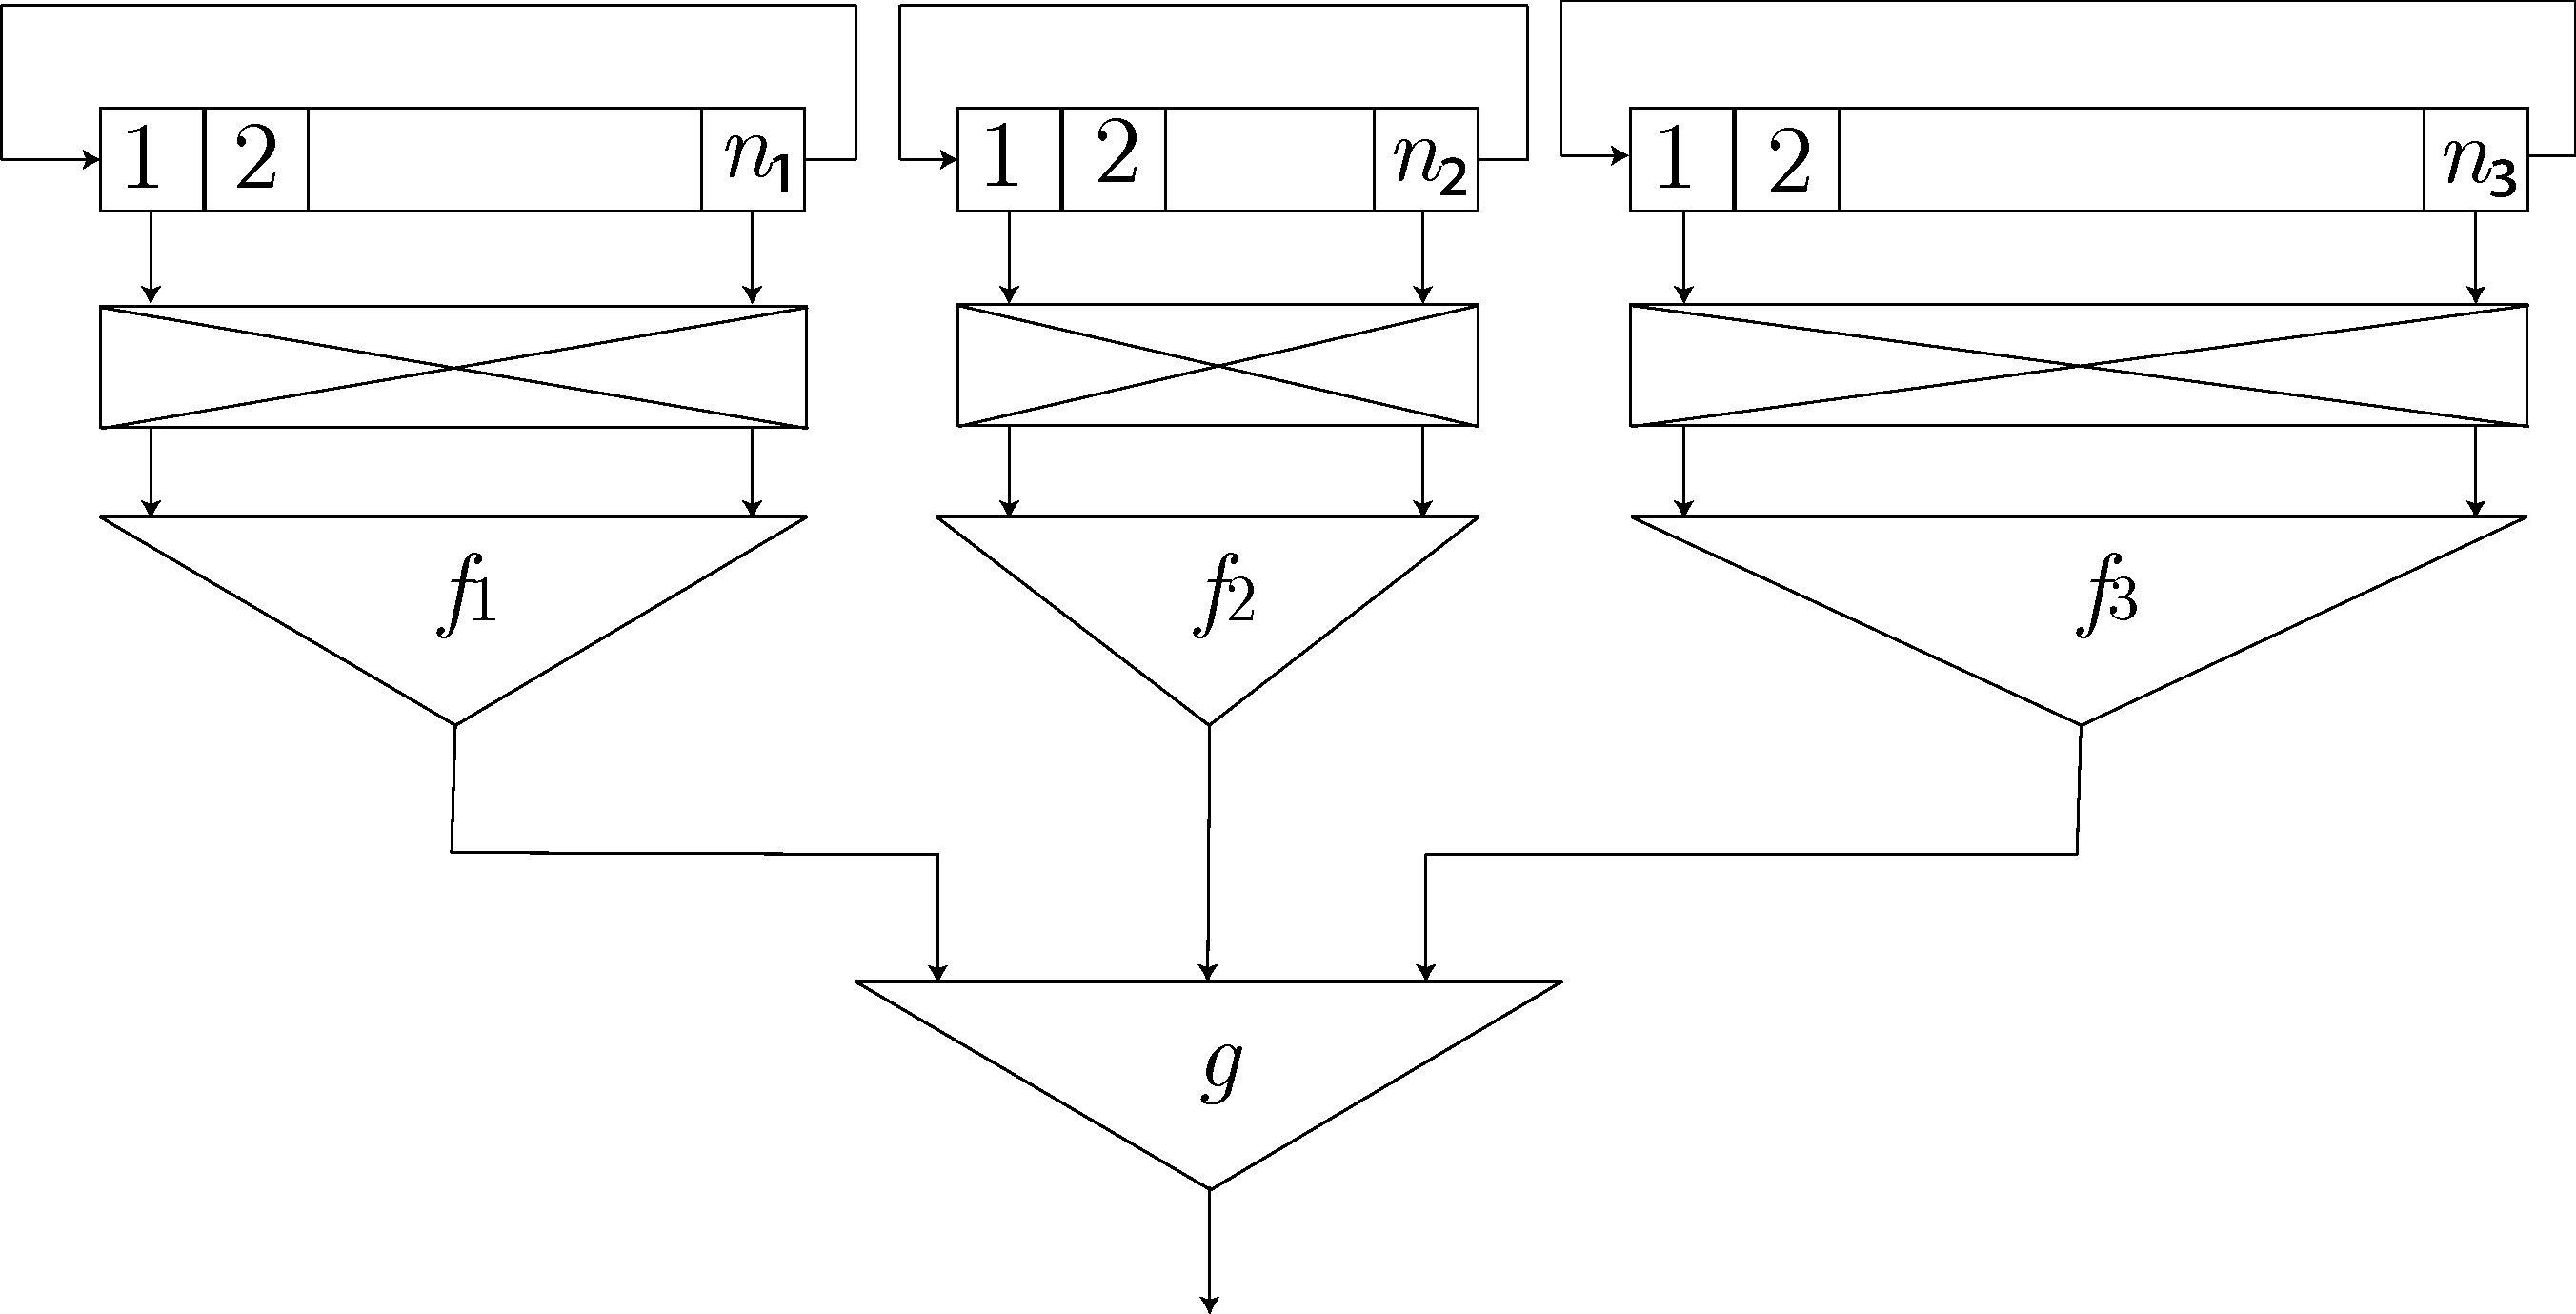
\includegraphics[width=\textwidth]{cipher}


	Поточный алгоритм шифрования типа «Раскольников» состоит из:
	
	\begin{enumerate}
	\item трех РСЛОС $L_i, i \in \overline{1,3}$, над полем $\mathbb{F}_2$ c характеристическими многочленами
	$F_1(x), F_2(x), F_3(x)$ степени соответственно $n_1, n_2, n_3$.
	
	\item трех коммутаторов (перестановок) $K_i, i \in \overline{1,3}, Ki \in S (l_i)$, на вход коммутатору $K_i$
	подаются значения РСЛОС $L_i$ с индексами
	\[ 1 = p1 < p2 < \dots < p_{l_i-1} < p_{l_i} = n_i \]

	\item трех функций усложнения выхода РСЛОС $f_i (x_1, x_2, \dots, x_{l_i}), i \in \overline{1,3},$ 
	
	\item комбинирующей булевой функции $g(x,y,z)$, задаваемой формулой ($\land$ -- <<и>>, $\neg$ -- отрицание, $\lor$ -- <<или>>, $\veebar$ -- <<исключающее или>>):
	\[ g(x,y,z) = (\neg x \lor \neg y) \land (x \lor y \lor \neg z) \land (\neg y \lor z) \]
	
	\end{enumerate}

	Ключом являются:
	
	\begin{itemize}[topsep=0pt, itemsep=0pt, parsep=0pt]
	\item начальное заполнение регистра $L_1$
	\item коммутатор $K_2$
	\item начальное заполнение регистра $L_3$
	\end{itemize}

	\section{Исследование ключевого множества}
	
	Множетсво ключей $K$ состоит из всезможожных троек вида $(k_1, k_2, k_3)$, где 
	
	\begin{itemize}[topsep=0pt, itemsep=0pt, parsep=0pt]
	\item $k_1$ - какое-то заполнение регистра $L_1$ длины $n_1$,
	\item $k_2$ - какая-то перестановка длины $n_2$, 
	\item $k_3$ - какое-то заполнение регистра $L_3$ длины $n_1$.
	\end{itemize}
	
	Тогда общее число ключей будет равно
	
	\[ |K| = 2^{n_1} \cdot n_2! \cdot 2^{n_3} \]
	
	Приведём пример параметров $n_1, n_2, n_3$, при котором $|K| > 2^{64}$. Пусть $n_1=25, n_2=10, n_3=25$, тогда
	
	\[ |K| = 2^{25} \cdot 10! \cdot 2^{25} > 2^{25} \cdot 2^{21} \cdot 2^{25} > 2^{71} > 2^{64} \]
	
	\section{Исследование узлов алгоритма}
	
	\subsection{Узлы РСЛОС}
	
	\textit{Регистр сдвига с линейной обратной связью} или \textit{РСЛОС} --- это блок, который генерирует двоичные псевдослучайные периодические последовательности, которые называются линейными рекуррентными последовательностями (ЛРП). 
	
	Широкое распространение в криптографических приложениях линейных регистров сдвига над конечными полями $\mathbb{F}_{2^n}$ и кольцами вычетов обусловлено целым рядом факторов. Среди них можно отметить:
	
	\begin{itemize}[topsep=0pt, itemsep=0pt, parsep=0pt]
		\item использование только простейших операций сложения и умножения, аппаратно реализованных практически на всех вычислительных средствах;
		\item высокое быстродействие создаваемых на их основе криптографических алгоритмов;
		\item большое количество теоретических исследований свойств линейных рекуррентных последовательностей (ЛРП), свидетельствующих об их удовлетворительных криптографических свойствах
	\end{itemize}

	В данном шифре в ключ входят только заполнения регистра сдвига, а вид характеристического многочлена, является параметром построения шифра. Значит, нужно подобрать такие функции обратной связи, чтобы для любого \textbf{ненулевого} заполнения ЛРП была максимального периода. В этом нам помогут следующие теормы и следствие из них.
	
	\begin{theorem}
		Пусть $u$ – ЛРП над полем $\mathbb{F}_q$ с реверсивным минимальным многочленом $F(x)$ степени $m$ и $q^m > 2$. Тогда следующие утверждения эквивалентны:
		\begin{enumerate}[topsep=0pt, itemsep=0pt, parsep=0pt, label=(\arabic*)]
			\item $u$ – ЛРП максимального периода;
			\item многочлен $F(x)$ неприводим над $\mathbb{F}_q$, и его корень $\alpha$ в минимальном поле разложения $\mathbb{F}_{q^m}$ над $\mathbb{F}_q$ есть примитивный элемент поля.
		\end{enumerate}
	\end{theorem}

	\begin{theorem}
		Неприводимый многочлен $F(x)$ примитивен в том и только в том случае, когда для любого простого числа $p$, делящего $q^m - 1$, 
		многочлен $x^{\frac{q^m - 1}{p}}$ не сравним с 1 по модулю многочлена $F(x)$.

	\end{theorem}
	
	\begin{corollary}
		Если $F(x)$ -- неприводимый многочлен над полем $\mathbb{F}_2$ степени $m$, и $2^m - 1$ -- простое число, то $F(x)$ -- примитивный многочлен.

	\end{corollary}

	Исходя из утверждений выше, для того чтобы линейная рекуррентная последовательность порядка $m$ над полем из $q$ элементов имела
	максимальный период, необходимо и достаточно, чтобы ее минимальный многочлен был примитивным многочленом.
	
	Более конкретно, над полем $\mathbb{F}_2$ необходимо реверсивный минимальный многочлен $F(x)$ на основе просых чисел Мерсенна. В этом случае для любого \textbf{ненулевого} заполнения ЛРП получается максимального периода.
	
	Приведём конкретный пример многочленов $F_1(x), F_2(x), F_3(x)$ для заданных нашим алгоритмом РСЛОС $L_1, L_2, L_3$. Для их генерации будем использовать втроенные функции пакета Wolfram Mathematica 
	
	Пусть $n_1=31, n_2=13, n_3=19$ ($2^{31}-1, 2^{13}-1$ и $2^{19}-1$ --- это известные числа Мерсенна).
	
	Пример неприодимых многочленов соотвествующих степеней из $\mathbb{F}_2$[x].
	\begin{align*}
		F_1(x) =& x^{31} + x^{30} + x^{29} + x^{28} + x^{27} + x^{24} + x^{21} + x^{19} + \\
			    &+ x^{18} + x^{13} + x^{12} + x^{10} + x^4 + x^3 + 1 \\[2ex]
		F_2(x) =& x^{13} + x^{12} + x^{11} + x^8 + x^7 + x^6 + x^5 + x^4 + x^2 + x + 1 \\[2ex]
		F_3(x) =& x^{19} + x^{15} + x^{13} + x^{12} + x^{10} + x^9 + x^5 + x^4 + x^2 + x + 1 
	\end{align*}
	
	В этом случае любое \textbf{ненулевое} заполнение каждого из $L_1, L_2, L_3$ даст нам максимальный период на каждом из регистрах. Кроме того, каждый регистр сдвига был выбран разной длинны для того, чтобы исключить случай совместного зацикливания двух ЛРП. Иными словами итоговый период совместной работы всех трёх регистров будет равна 
	
	\[ N_{L_1 L_2 L_3} = \text{НОК}(2^{n_1}-1, 2^{n_2}-1, 2^{n_3}-1) = \text{НОК}(2^{31}-1, 2^{13}-1, 2^{19}-1) \approx 2^{63} \]

	Это означает, что вектор начальных заполнений $(u_1, u_2, u_3)$ регистров $L_1, L_2, L_3$ вернётся в сам в себя после $N_{L_1 L_2 L_3} \approx 2^{63} $ совместных тактов работы всех трёх регистров.
	
	При этом мощность ключевого множества по-прежнему будет удовлетворять условию $|K| > 2^{64}$:
	
	\[ |K| = 2^{31} \cdot 13! \cdot 2^{19} > 2^{31} \cdot 2^{32} \cdot 2^{19} > 2^{82} > 2^{64} \]
	
	\subsection{Функции усложнения}
	
	Для усложнения аналитической сложности выходной	последовательности РСЛОС используются функции усложнения. «Фильтрующая» функция f должна выбираться так, чтобы выходная последовательность имела распределение, близкое к равномерному распределению, и высокую линейную сложность.

	
	Ниже представленые основные криптографические характеристики нелинейных преобразований, используемые в поточных шифрах.
	
	
	\begin{property}
		Функция $f$ фильтрующего генератора должна быть сбалансированной, т.е.  $|\{x : f(x) = 0\}| = 2^{n-1} $.  
	\end{property}

	\begin{property} \label{prop::zapr}
		У функция $f$ фильтрующего генератора должны отсуствовать запреты. 
	\end{property}

	Для выполненеия свойтсва \ref{prop::zapr} достаточно, чтобы функция $f$ была линейна по крайней переменной. Есть более общий критерий определения имеет ли булева фунция запрет или нет.
	
	\begin{theorem}
		Булева функция не имеет запрета тогда и только тогда, когда она сильно равновероятна.

	\end{theorem}

	\begin{property} 
		У функция $f$ фильтрующего генератора должна иметь высокую алгебраическую степень.
	\end{property}

	\begin{property} 
		Функция $f$ фильтрующего генератора должна иметь высокую нелинейность, т.е. не иметь эффективных линейных статистических аналогов.
	\end{property}

	\begin{property} 
		Функция $f$ фильтрующего генератора должна быть $k$\-/равновероятной для максимально возможного значения $k$.
	\end{property}
	
	\begin{property} 
		Функция $f$ фильтрующего генератора (а также функция $f~+~1$) не должны иметь аннигиляторов малой алгебраической степени.
	\end{property}
	
	
	На практикте помимо достежния перечисленных условий необходимо дополнительно исследовать весь блок фильтрующего гереатора целиком.
	Например, фильтрующий генератор с нелинейной функцией усложнения может представляться в виде ЛРП с меньшим (чем исходная ЛРП) периодом.
	
	В работе \textcite{rachwalik2012generation} были найдены несколько функций усложнения порядков 25 и 27. Работа была нацелена на поиск таких фукнций, что обеспечивают наибольший период выходной последовательности. Кроме того у перечисленных в работе булевых функций были ислледованы некоторые статистические свойства выходных последовательностей. Возьмём эти функции усложнения за основу, приняв некоторые переменные за единицу.
	
	\begin{align*}
		f_1 =& x_0 \oplus x_6 \oplus x_{11} \oplus x_{14} \oplus x_{16} \oplus x_{17} \oplus x_{18} \oplus x_{19} \oplus x_{23} \oplus\\
			 &\oplus x_{4} x_{19} \oplus x_{4} x_{21} \oplus x_5 x_{22} \oplus x_9 x_{19} \oplus x_1 x_{17} x_23 \oplus x_5 x_7 x_{18} \oplus x_5 x_{12} x_{19} \\[2ex]
		f_2 =& x_0 \oplus x_3 \oplus x_6 \oplus x_{10} \oplus x_6 x_9 \oplus x_6 x_{10}
\oplus x_4 x_9 x_{10} \\[2ex]
		f_3 =& x_0 \oplus x_8 \oplus x_9 \oplus x_{10} \oplus x_{11} \oplus x_{10} x_{14} \oplus x_4 x_{16}\oplus x_{11} x_{16} \oplus x_1 x_5 x_7 
	\end{align*}
	
	
	
	
		
\end{document}